* Distancia a algunos conceptos de estado y revolución
% 
    \begin{center}
      \begin{tabular}{ | l | l | l |}
        \hline
        Choosen Sensens & Closest Top Sense & similarity  \\ \hline
\multicolumn{3}{|c|}{The State and Revolution - path similarity} \\ \hline
revolution.n.01 & revolution.n.01 & 1.0 \\ \hline
imperialism.n.02 & communism.n.02 & 0.333333333333 \\ \hline
proletarian.n.01 & peer.n.01 & 0.25 \\ \hline
practice.n.03 & work.n.01 & 0.2 \\ \hline
toilet.n.04 & work.n.01 & 0.166666666667 \\ \hline
war.n.01 & work.n.01 & 0.166666666667 \\ \hline
money.n.01 & phase.n.01 & 0.125 \\ \hline
philosophy.n.02 & law.n.04 & 0.125 \\ \hline
materialism.n.02 & law.n.04 & 0.125 \\ \hline
strategy.n.02 & law.n.04 & 0.125 \\ \hline
idealism.n.01 & law.n.04 & 0.125 \\ \hline
capitalism.n.01 & democracy.n.02 & 0.125 \\ \hline
hair.n.01 & peer.n.01 & 0.111111111111 \\ \hline
theory.n.01 & experience.n.03 & 0.1 \\ \hline
television receiver.n.01 & peer.n.01 & 0.0833333333333 \\ \hline
car.n.01 & peer.n.01 & 0.0833333333333 \\ \hline
lion.n.01 & peer.n.01 & 0.0833333333333 \\ \hline
sugar.n.01 & peer.n.01 & 0.0833333333333 \\ \hline
\multicolumn{3}{|c|}{The State and Revolution - lch similarity} \\ \hline
revolution.n.01 & revolution.n.01 & 3.63758615973 \\ \hline
imperialism.n.02 & communism.n.02 & 2.53897387106 \\ \hline
proletarian.n.01 & peer.n.01 & 2.25129179861 \\ \hline
practice.n.03 & work.n.01 & 2.02814824729 \\ \hline
toilet.n.04 & work.n.01 & 1.8458266905 \\ \hline
war.n.01 & work.n.01 & 1.8458266905 \\ \hline
money.n.01 & phase.n.01 & 1.55814461805 \\ \hline
philosophy.n.02 & law.n.04 & 1.55814461805 \\ \hline
materialism.n.02 & law.n.04 & 1.55814461805 \\ \hline
strategy.n.02 & law.n.04 & 1.55814461805 \\ \hline
idealism.n.01 & law.n.04 & 1.55814461805 \\ \hline
capitalism.n.01 & democracy.n.02 & 1.55814461805 \\ \hline
hair.n.01 & peer.n.01 & 1.44036158239 \\ \hline
theory.n.01 & experience.n.03 & 1.33500106673 \\ \hline
television receiver.n.01 & peer.n.01 & 1.15267950994 \\ \hline
car.n.01 & peer.n.01 & 1.15267950994 \\ \hline
lion.n.01 & peer.n.01 & 1.15267950994 \\ \hline
sugar.n.01 & peer.n.01 & 1.15267950994 \\ \hline
\multicolumn{3}{|c|}{The State and Revolution - res similarity} \\ \hline
revolution.n.01 & revolution.n.01 & 10.3880624692 \\ \hline
imperialism.n.02 & communism.n.02 & 8.60196873746 \\ \hline
philosophy.n.02 & law.n.04 & 3.29228159341 \\ \hline
materialism.n.02 & law.n.04 & 3.29228159341 \\ \hline
strategy.n.02 & law.n.04 & 3.29228159341 \\ \hline
idealism.n.01 & law.n.04 & 3.29228159341 \\ \hline
toilet.n.04 & work.n.01 & 3.14352023311 \\ \hline
capitalism.n.01 & club.n.02 & 2.85529368615 \\ \hline
money.n.01 & phase.n.01 & 2.69110280536 \\ \hline
theory.n.01 & law.n.04 & 2.64452085446 \\ \hline
proletarian.n.01 & engels.n.01 & 2.33354524374 \\ \hline
war.n.01 & work.n.01 & 2.33223775508 \\ \hline
practice.n.03 & work.n.01 & 2.33223775508 \\ \hline
lion.n.01 & engels.n.01 & 2.22415047123 \\ \hline
television receiver.n.01 & engels.n.01 & 1.53183374322 \\ \hline
car.n.01 & engels.n.01 & 1.53183374322 \\ \hline
hair.n.01 & engels.n.01 & 1.53183374322 \\ \hline
sugar.n.01 & engels.n.01 & 0.801759114954 \\ \hline
\multicolumn{3}{|c|}{The State and Revolution - jcn similarity} \\ \hline
revolution.n.01 & revolution.n.01 & 1e+300 \\ \hline
imperialism.n.02 & communism.n.02 & 0.14975874591 \\ \hline
war.n.01 & work.n.01 & 0.119881984187 \\ \hline
philosophy.n.02 & law.n.04 & 0.103411969458 \\ \hline
practice.n.03 & work.n.01 & 0.103154641506 \\ \hline
toilet.n.04 & work.n.01 & 0.0985118809398 \\ \hline
money.n.01 & phase.n.01 & 0.0916158054473 \\ \hline
theory.n.01 & work.n.01 & 0.0910758552239 \\ \hline
car.n.01 & peer.n.01 & 0.0887294617483 \\ \hline
hair.n.01 & peer.n.01 & 0.0868826421077 \\ \hline
proletarian.n.01 & peer.n.01 & 0.0849595683478 \\ \hline
strategy.n.02 & law.n.04 & 0.07841412673 \\ \hline
lion.n.01 & peer.n.01 & 0.0750424463326 \\ \hline
television receiver.n.01 & peer.n.01 & 0.0731074093034 \\ \hline
capitalism.n.01 & club.n.02 & 0.0729022081709 \\ \hline
materialism.n.02 & law.n.04 & 0.0719531280061 \\ \hline
idealism.n.01 & law.n.04 & 0.0678185221973 \\ \hline
sugar.n.01 & work.n.01 & 0.0625959407953 \\ \hline
\multicolumn{3}{|c|}{The State and Revolution - lin similarity} \\ \hline
revolution.n.01 & revolution.n.01 & 1.0 \\ \hline
imperialism.n.02 & communism.n.02 & 0.720392353354 \\ \hline
philosophy.n.02 & law.n.04 & 0.405088626962 \\ \hline
toilet.n.04 & work.n.01 & 0.382467580972 \\ \hline
war.n.01 & work.n.01 & 0.35863993877 \\ \hline
strategy.n.02 & law.n.04 & 0.340509805473 \\ \hline
money.n.01 & phase.n.01 & 0.330250297796 \\ \hline
practice.n.03 & work.n.01 & 0.324854541172 \\ \hline
materialism.n.02 & law.n.04 & 0.321472637881 \\ \hline
idealism.n.01 & law.n.04 & 0.308702564543 \\ \hline
theory.n.01 & law.n.04 & 0.305328480717 \\ \hline
capitalism.n.01 & club.n.02 & 0.29394209418 \\ \hline
proletarian.n.01 & peer.n.01 & 0.28393127113 \\ \hline
lion.n.01 & peer.n.01 & 0.250268807542 \\ \hline
car.n.01 & peer.n.01 & 0.213736072979 \\ \hline
hair.n.01 & peer.n.01 & 0.210222579299 \\ \hline
television receiver.n.01 & peer.n.01 & 0.182991045418 \\ \hline
sugar.n.01 & peer.n.01 & 0.0895207954547 \\ \hline
\end{tabular}
\end{center}

For each work we executed the algorithm and then we obtained five different similarities for the top senses.
We compared the similarity of top sense against each other and against a list handpicked synsets \ref{handpicked_synsets}

First we show the results obtained after the execution for some works , then we analyze the results of similarity.

\begin{table}[h!]
    \begin{center}
        \begin{tabular}{ | L{2cm} | L{5cm} |}
            \hline
            Synset & Gloss \\ \hline
            \multicolumn{2}{|c|}{Human handpicked concepts to compare against top senses} \\ \hline
war & the waging of armed conflict against an enemy \\ \hline
capitalism & an economic system based on private ownership of capital\\ \hline
theory & a well-substantiated explanation of some aspect of the natural world \\ \hline
toilet & the act of dressing and preparing yourself \\ \hline
imperialism & a political orientation that advocates imperial interests \\ \hline
proletarian & a member of the working class (not necessarily employed) \\ \hline
practice & translating an idea into action \\ \hline
revolution & a drastic and far-reaching change in ways of thinking and behaving \\ \hline
money & the most common medium of exchange; functions as legal tender \\ \hline
philosophy & the rational investigation of questions about existence and knowledge and ethics \\ \hline
idealism & (philosophy) the philosophical theory that ideas are the only reality \\ \hline
strategy & the branch of military science dealing with military command and the planning and conduct of a war \\ \hline
materialism & (philosophy) the philosophical theory that matter is the only reality \\ \hline
lion & large gregarious predatory feline of Africa and India having a tawny coat with a shaggy mane in the male \\ \hline
television_receiver. & an electronic device that receives television signals and displays them on a screen \\ \hline
hair & a covering for the body (or parts of it) consisting of a dense growth of threadlike structures (as on the human head); helps to prevent heat loss \\ \hline
sugar & a white crystalline carbohydrate used as a sweetener and preservative \\ \hline
car & a motor vehicle with four wheels; usually propelled by an internal combustion engine \\ \hline
            \multicolumn{2}{|c|}{Categories} \\ \hline
economy & the system of production and distribution and consumption \\ \hline
philosophy & the rational investigation of questions about existence and knowledge and ethics \\ \hline
politics & social relations involving intrigue to gain authority or power \\ \hline
        \end{tabular}
    \end{center}
    \label{table:handpicked_synsets}
    \caption{Caption test}
\end{table}


\begin{table}[h!]
    \begin{center}
        \begin{tabular}{ | L{2cm} | L{5cm} |}
            \hline
            Top Sense & Sense Detected \\ \hline
            \multicolumn{2}{|c|}{The State and Revolution} \\ \hline
    engels & socialist who wrote the Communist Manifesto with Karl Marx in 1848 (1820-1895) \\ \hline
    work & activity directed toward making or doing something \\ \hline
    club & a formal association of people with similar interests \\ \hline
    democracy & a political system in which the supreme power lies in a body of citizens who can elect people to represent them \\ \hline
            \multicolumn{2}{|c|}{MATERIALISM and EMPIRIO} \\ \hline
    physics & the science of matter and energy and their interactions \\ \hline
    sociable & a party of people assembled to promote sociability and communal activity \\ \hline
    kant & influential German idealist philosopher (1724-1804) \\ \hline
    time & the continuum of experience in which events pass from the future through the present to the past \\ \hline
    space & an empty area (usually bounded in some way between things) \\ \hline
            \multicolumn{2}{|c|}{Imperialism, the highest stage of capitalism} \\ \hline
 enterprise & an organization created for business ventures \\ \hline
 depository\_financial\_institution & a financial institution that accepts deposits and channels the money into lending activities \\ \hline
 depository\_financial\_institution & a financial institution that accepts deposits and channels the money into lending activities \\ \hline
 imperialism & a policy of extending your rule over foreign countries \\ \hline
 universe & everything that exists anywhere \\ \hline
        \end{tabular}
    \end{center}
    \label{table:top_senses}
    \caption{Caption test}
\end{table}

In the next Table we can observe the best top sense matches for our handpicked synsets.

    \begin{center}
      \begin{tabular}{ | l | l | l |}
        \hline
        Choosen Sensens & Closest Top Sense & similarity  \\ \hline
\multicolumn{3}{|c|}{The State and Revolution - path similarity} \\ \hline
revolution.n.01 & revolution.n.01 & 1.0 \\ \hline
imperialism.n.02 & communism.n.02 & 0.333333333333 \\ \hline
proletarian.n.01 & peer.n.01 & 0.25 \\ \hline
practice.n.03 & work.n.01 & 0.2 \\ \hline
toilet.n.04 & work.n.01 & 0.166666666667 \\ \hline
war.n.01 & work.n.01 & 0.166666666667 \\ \hline
money.n.01 & phase.n.01 & 0.125 \\ \hline
philosophy.n.02 & law.n.04 & 0.125 \\ \hline
materialism.n.02 & law.n.04 & 0.125 \\ \hline
strategy.n.02 & law.n.04 & 0.125 \\ \hline
idealism.n.01 & law.n.04 & 0.125 \\ \hline
capitalism.n.01 & democracy.n.02 & 0.125 \\ \hline
hair.n.01 & peer.n.01 & 0.111111111111 \\ \hline
theory.n.01 & experience.n.03 & 0.1 \\ \hline
television receiver.n.01 & peer.n.01 & 0.0833333333333 \\ \hline
car.n.01 & peer.n.01 & 0.0833333333333 \\ \hline
lion.n.01 & peer.n.01 & 0.0833333333333 \\ \hline
sugar.n.01 & peer.n.01 & 0.0833333333333 \\ \hline
\multicolumn{3}{|c|}{The State and Revolution - lch similarity} \\ \hline
revolution.n.01 & revolution.n.01 & 3.63758615973 \\ \hline
imperialism.n.02 & communism.n.02 & 2.53897387106 \\ \hline
proletarian.n.01 & peer.n.01 & 2.25129179861 \\ \hline
practice.n.03 & work.n.01 & 2.02814824729 \\ \hline
toilet.n.04 & work.n.01 & 1.8458266905 \\ \hline
war.n.01 & work.n.01 & 1.8458266905 \\ \hline
money.n.01 & phase.n.01 & 1.55814461805 \\ \hline
philosophy.n.02 & law.n.04 & 1.55814461805 \\ \hline
materialism.n.02 & law.n.04 & 1.55814461805 \\ \hline
strategy.n.02 & law.n.04 & 1.55814461805 \\ \hline
idealism.n.01 & law.n.04 & 1.55814461805 \\ \hline
capitalism.n.01 & democracy.n.02 & 1.55814461805 \\ \hline
hair.n.01 & peer.n.01 & 1.44036158239 \\ \hline
theory.n.01 & experience.n.03 & 1.33500106673 \\ \hline
television receiver.n.01 & peer.n.01 & 1.15267950994 \\ \hline
car.n.01 & peer.n.01 & 1.15267950994 \\ \hline
lion.n.01 & peer.n.01 & 1.15267950994 \\ \hline
sugar.n.01 & peer.n.01 & 1.15267950994 \\ \hline
\multicolumn{3}{|c|}{The State and Revolution - res similarity} \\ \hline
revolution.n.01 & revolution.n.01 & 10.3880624692 \\ \hline
imperialism.n.02 & communism.n.02 & 8.60196873746 \\ \hline
philosophy.n.02 & law.n.04 & 3.29228159341 \\ \hline
materialism.n.02 & law.n.04 & 3.29228159341 \\ \hline
strategy.n.02 & law.n.04 & 3.29228159341 \\ \hline
idealism.n.01 & law.n.04 & 3.29228159341 \\ \hline
toilet.n.04 & work.n.01 & 3.14352023311 \\ \hline
capitalism.n.01 & club.n.02 & 2.85529368615 \\ \hline
money.n.01 & phase.n.01 & 2.69110280536 \\ \hline
theory.n.01 & law.n.04 & 2.64452085446 \\ \hline
proletarian.n.01 & engels.n.01 & 2.33354524374 \\ \hline
war.n.01 & work.n.01 & 2.33223775508 \\ \hline
practice.n.03 & work.n.01 & 2.33223775508 \\ \hline
lion.n.01 & engels.n.01 & 2.22415047123 \\ \hline
television receiver.n.01 & engels.n.01 & 1.53183374322 \\ \hline
car.n.01 & engels.n.01 & 1.53183374322 \\ \hline
hair.n.01 & engels.n.01 & 1.53183374322 \\ \hline
sugar.n.01 & engels.n.01 & 0.801759114954 \\ \hline
\multicolumn{3}{|c|}{The State and Revolution - jcn similarity} \\ \hline
revolution.n.01 & revolution.n.01 & 1e+300 \\ \hline
imperialism.n.02 & communism.n.02 & 0.14975874591 \\ \hline
war.n.01 & work.n.01 & 0.119881984187 \\ \hline
philosophy.n.02 & law.n.04 & 0.103411969458 \\ \hline
practice.n.03 & work.n.01 & 0.103154641506 \\ \hline
toilet.n.04 & work.n.01 & 0.0985118809398 \\ \hline
money.n.01 & phase.n.01 & 0.0916158054473 \\ \hline
theory.n.01 & work.n.01 & 0.0910758552239 \\ \hline
car.n.01 & peer.n.01 & 0.0887294617483 \\ \hline
hair.n.01 & peer.n.01 & 0.0868826421077 \\ \hline
proletarian.n.01 & peer.n.01 & 0.0849595683478 \\ \hline
strategy.n.02 & law.n.04 & 0.07841412673 \\ \hline
lion.n.01 & peer.n.01 & 0.0750424463326 \\ \hline
television receiver.n.01 & peer.n.01 & 0.0731074093034 \\ \hline
capitalism.n.01 & club.n.02 & 0.0729022081709 \\ \hline
materialism.n.02 & law.n.04 & 0.0719531280061 \\ \hline
idealism.n.01 & law.n.04 & 0.0678185221973 \\ \hline
sugar.n.01 & work.n.01 & 0.0625959407953 \\ \hline
\multicolumn{3}{|c|}{The State and Revolution - lin similarity} \\ \hline
revolution.n.01 & revolution.n.01 & 1.0 \\ \hline
imperialism.n.02 & communism.n.02 & 0.720392353354 \\ \hline
philosophy.n.02 & law.n.04 & 0.405088626962 \\ \hline
toilet.n.04 & work.n.01 & 0.382467580972 \\ \hline
war.n.01 & work.n.01 & 0.35863993877 \\ \hline
strategy.n.02 & law.n.04 & 0.340509805473 \\ \hline
money.n.01 & phase.n.01 & 0.330250297796 \\ \hline
practice.n.03 & work.n.01 & 0.324854541172 \\ \hline
materialism.n.02 & law.n.04 & 0.321472637881 \\ \hline
idealism.n.01 & law.n.04 & 0.308702564543 \\ \hline
theory.n.01 & law.n.04 & 0.305328480717 \\ \hline
capitalism.n.01 & club.n.02 & 0.29394209418 \\ \hline
proletarian.n.01 & peer.n.01 & 0.28393127113 \\ \hline
lion.n.01 & peer.n.01 & 0.250268807542 \\ \hline
car.n.01 & peer.n.01 & 0.213736072979 \\ \hline
hair.n.01 & peer.n.01 & 0.210222579299 \\ \hline
television receiver.n.01 & peer.n.01 & 0.182991045418 \\ \hline
sugar.n.01 & peer.n.01 & 0.0895207954547 \\ \hline
\end{tabular}
\end{center}

After a careful analysis of out results we found some problems with pronouns that we show in \ref{table:pronouns}
We think that this mismatch could be a cause of our Lesk algorithm modification to check against to context words directly.

\begin{table}[h!]
    \begin{center}
        \begin{tabular}{ | L{3cm} | L{1cm} | L{3cm} |}
            \hline
            Text &  Top Sense & Sense Detected \\ \hline
            \multicolumn{3}{|c|}{Strange detections} \\ \hline
    The Agrarian Programme & marx & United States comedian; one of four brothers who made motion pictures together (1901-1979) \\ \hline

    The State and Revolution & bernstein & United States conductor and composer (1918-1990) \\ \hline
        \end{tabular}
    \end{center}
    \caption{Caption test}
    \label{table:pronouns}
\end{table}


One interesting thing to observe is the distance between the all the top senses of all texts.

\begin{figure}[h!]
    \caption{Top senses lch distance of all Lenin works.}
    \centering
    
\includegraphics[width=0.5\textwidth]{lch_sim_graph.png}
    \label{fig:lch_sim_graph}
\end{figure}



Now our question is. how far are the top senses from the concepts we wanted to compare to?
To answer that question we find interesting to study what happens if we add pylosophical, political and economic senses in out graph and calculate form those synsets the similarity to top senses.



\begin{figure}[h!]
    \caption{Top senses against economy philosophy and politics using LCH similarity}
    \centering
    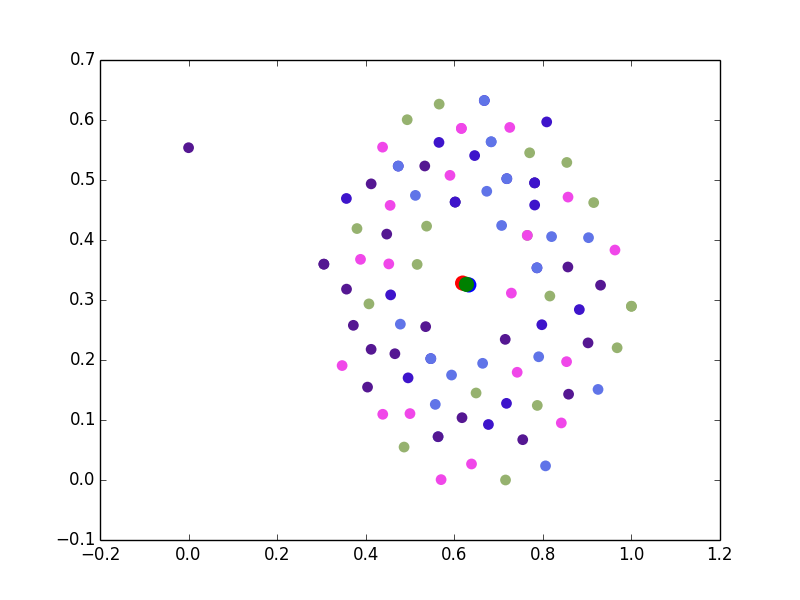
\includegraphics[width=0.5\textwidth]{phyl_eco_pol_lch_sim_graph.png}
    \label{fig:phyl_eco_pol_lch_sim_graph}
\end{figure}

At ~\ref{fig:phyl_eco_pol_lch_sim_graph} we notw that the synsets phylosophy, economic and politics are very close to each other

We tried several similarity measures and most of them gave that phylosophy, economic and politics are similar synsets.
However when we tried JCN similarity we found that those synsets were far enough from each other \ref{fig:phyl_eco_pol_jcn_sim_graph}. We can\'t get any concise results since nodes in \ref{fig:phyl_eco_pol_jcn_sim_graph} seems to be very dispersed.

\begin{figure}[h!]
    \caption{Top senses against economy philosophy and politics using JCN similarity}
    \centering
    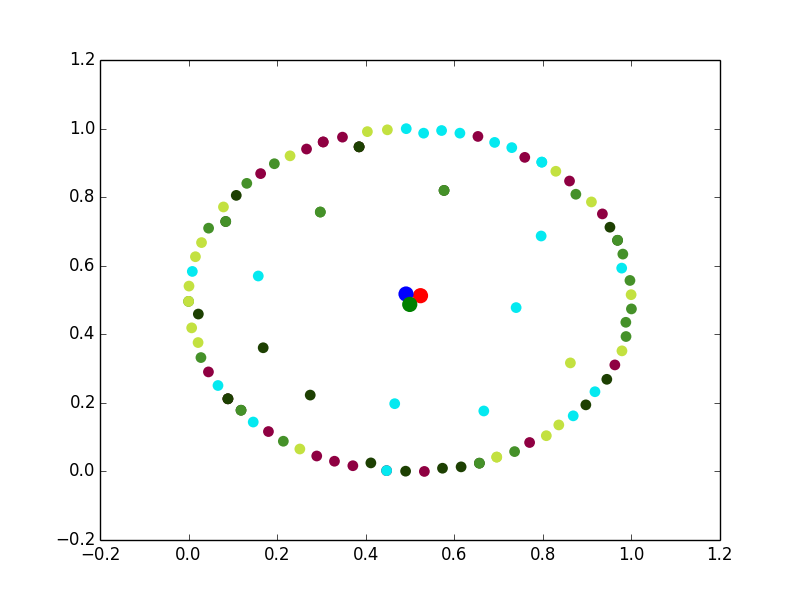
\includegraphics[width=0.5\textwidth]{phyl_eco_pol_jcn_sim_graph.png}
    \label{fig:phyl_eco_pol_jcn_sim_graph}
\end{figure}

FALTAN LOS GRAFICOS DE LOS HANDPICKED
